


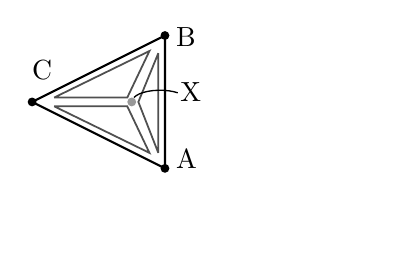
\begin{tikzpicture}[y=0.80pt, x=0.8pt,yscale=-1, inner sep=0pt, outer sep=0pt]
\begin{scope}[shift={(-16.10332,-41.20103)}]
  \path[fill=black] (178.797,148.02312) node[above right] (text6246) {};
  \path[shift={(16.10332,-258.79897)},fill=black,nonzero rule] (12.0000,340.0000)
    .. controls (12.0000,341.1046) and (11.1046,342.0000) .. (10.0000,342.0000) ..
    controls (8.8954,342.0000) and (8.0000,341.1046) .. (8.0000,340.0000) ..
    controls (8.0000,338.8954) and (8.8954,338.0000) .. (10.0000,338.0000) ..
    controls (11.1046,338.0000) and (12.0000,338.8954) .. (12.0000,340.0000) --
    cycle;
  \path[shift={(76.10332,-288.79897)},fill=black,nonzero rule] (12.0000,340.0000)
    .. controls (12.0000,341.1046) and (11.1046,342.0000) .. (10.0000,342.0000) ..
    controls (8.8954,342.0000) and (8.0000,341.1046) .. (8.0000,340.0000) ..
    controls (8.0000,338.8954) and (8.8954,338.0000) .. (10.0000,338.0000) ..
    controls (11.1046,338.0000) and (12.0000,338.8954) .. (12.0000,340.0000) --
    cycle;
  \path[shift={(76.10332,-228.79897)},fill=black,nonzero rule] (12.0000,340.0000)
    .. controls (12.0000,341.1046) and (11.1046,342.0000) .. (10.0000,342.0000) ..
    controls (8.8954,342.0000) and (8.0000,341.1046) .. (8.0000,340.0000) ..
    controls (8.0000,338.8954) and (8.8954,338.0000) .. (10.0000,338.0000) ..
    controls (11.1046,338.0000) and (12.0000,338.8954) .. (12.0000,340.0000) --
    cycle;
  \path[shift={(61.10332,-258.79897)},fill=black,fill opacity=0.404,nonzero rule]
    (12.0000,340.0000) .. controls (12.0000,341.1046) and (11.1046,342.0000) ..
    (10.0000,342.0000) .. controls (8.8954,342.0000) and (8.0000,341.1046) ..
    (8.0000,340.0000) .. controls (8.0000,338.8954) and (8.8954,338.0000) ..
    (10.0000,338.0000) .. controls (11.1046,338.0000) and (12.0000,338.8954) ..
    (12.0000,340.0000) -- cycle;
  \path[fill=black] (91.103317,111.20103) node[above right] (text3133) {A};
  \path[fill=black] (91.103317,56.201031) node[above right] (text3137) {B};
  \path[fill=black] (26.103317,71.201027) node[above right] (text3141) {C};
  \path[shift={(16.10332,-18.79897)},draw=black,line join=miter,line cap=butt,line
    width=0.800pt] (10.0000,100.0000) -- (70.0000,70.0000) -- (70.0000,130.0000)
    -- cycle;
  \path[shift={(16.10332,-18.79897)},draw=black,line join=miter,line
    cap=butt,miter limit=4.00,draw opacity=0.686,line width=0.640pt]
    (20.0000,98.0000) -- (63.0000,77.0000) -- (53.0000,98.0000) -- cycle;
  \path[shift={(16.10332,-18.79897)},draw=black,line join=miter,line
    cap=butt,miter limit=4.00,draw opacity=0.686,line width=0.640pt]
    (67.0000,78.0000) -- (58.0000,100.0000) -- (67.0000,123.0000) -- cycle;
  \path[shift={(16.10332,-18.79897)},draw=black,line join=miter,line
    cap=butt,miter limit=4.00,draw opacity=0.686,line width=0.640pt]
    (20.0000,102.0000) -- (53.0000,102.0000) -- (63.0000,123.0000) -- cycle;
  \path[fill=black] (93.103317,81.201027) node[above right] (text3157) {X};
  \path[shift={(-8.65052,-9.08887)},draw=black,fill=black,line join=round,miter
    limit=4.00,fill opacity=0.000,nonzero rule,line width=0.480pt]
    (80.7538,88.2899) .. controls (83.1150,85.6950) and (90.2880,84.3571) ..
    (96.7753,85.3015) .. controls (98.1455,85.5010) and (99.4178,85.7949) ..
    (100.5349,86.1698);
\end{scope}

\end{tikzpicture}

